%
% File lastname_firstname_title.tex
%
% Contact: dkdougal@byu.edu
%%
%% Based on the style files for ACL-2015 and ACL-2019

\documentclass[11pt,table,xcdraw]{article}
\usepackage[hyperref]{tex_styles/acl2019_no_nums}

\usepackage{import}
\usepackage{booktabs}
\usepackage{float}
\import{./}{tex_styles/preamble.tex}

\graphicspath{{images/}}

\setlength\titlebox{5 cm}

% Turn off hyphenation
%\hyphenpenalty=10000
%\exhyphenpenalty=10000

\title{Blank Template for LING 581 Research Paper--Your Title Goes Here}

\author{Isaiah Pettingill \\
  Linguistics 581, Section 002, Winter 2026 \\
  Submitted to Professor Vasicek \\
  Department of Linguistics \\
  Brigham Young University \\
  {\tt isaiahjp@byu.edu} }

\begin{document}

\maketitle

\begin{abstract}
A brief summary of the research, including the purpose, methods, results, and conclusions.

[For your final paper submission, you may use an AI-generated summary of your manuscript \textit{for the Abstract section only} so long as you cite the proper AI attribution like this ~\cite{gpt53codex}.]
\end{abstract}

\section{Introduction}
Sentiment Analysis of free form text is useful across many domains. It is used for analyzing incoming consumer data through CX and EX touchpoints (such as employer ratings, consumer reviews, CSAT surveys, etc.), in the medical space, in mass-analyzing public sentiment on certain topics via social media, and in more complex flows that identify individual emotions. Numerical ratings are easy to process, but free-form text is traditionally harder to process with the possibility of being more useful.

In recent years, both Specialized Sentiment Analysis Models and Large Language Models (LLMs) have become increasingly powerful and increasingly low-cost, to the point that they can be run on consumer hardware or cheap cloud compute at a much larger scale. Many current sentiment analysis models are built on the same transformers architecture that powers LLMs but are made to perform a single task with high accuracy and a smaller number of parameters. LLMs have a better understanding of language in general, and are often advocated for as a solution to the issues of nuanced sentiment analysis across domains. It can be cheaper to implement an LLM-based classification flow when the team doesn't have the expertise to train a specialized model on their domain and want general, good results without the overhead of specialization, however the compute costs of LLMs at a large scale may quickly overcome that.

In the last few months, both Alibaba and Google have released competitive open-source LLMs that are on par with many leading models of similar weight classes. These models have intelligence comparable to or greater than GPT-4o at much smaller parameter sizes. In some cases, outperforming leading models on hallucinations and other metric.

\begin{figure}[H]
\centering
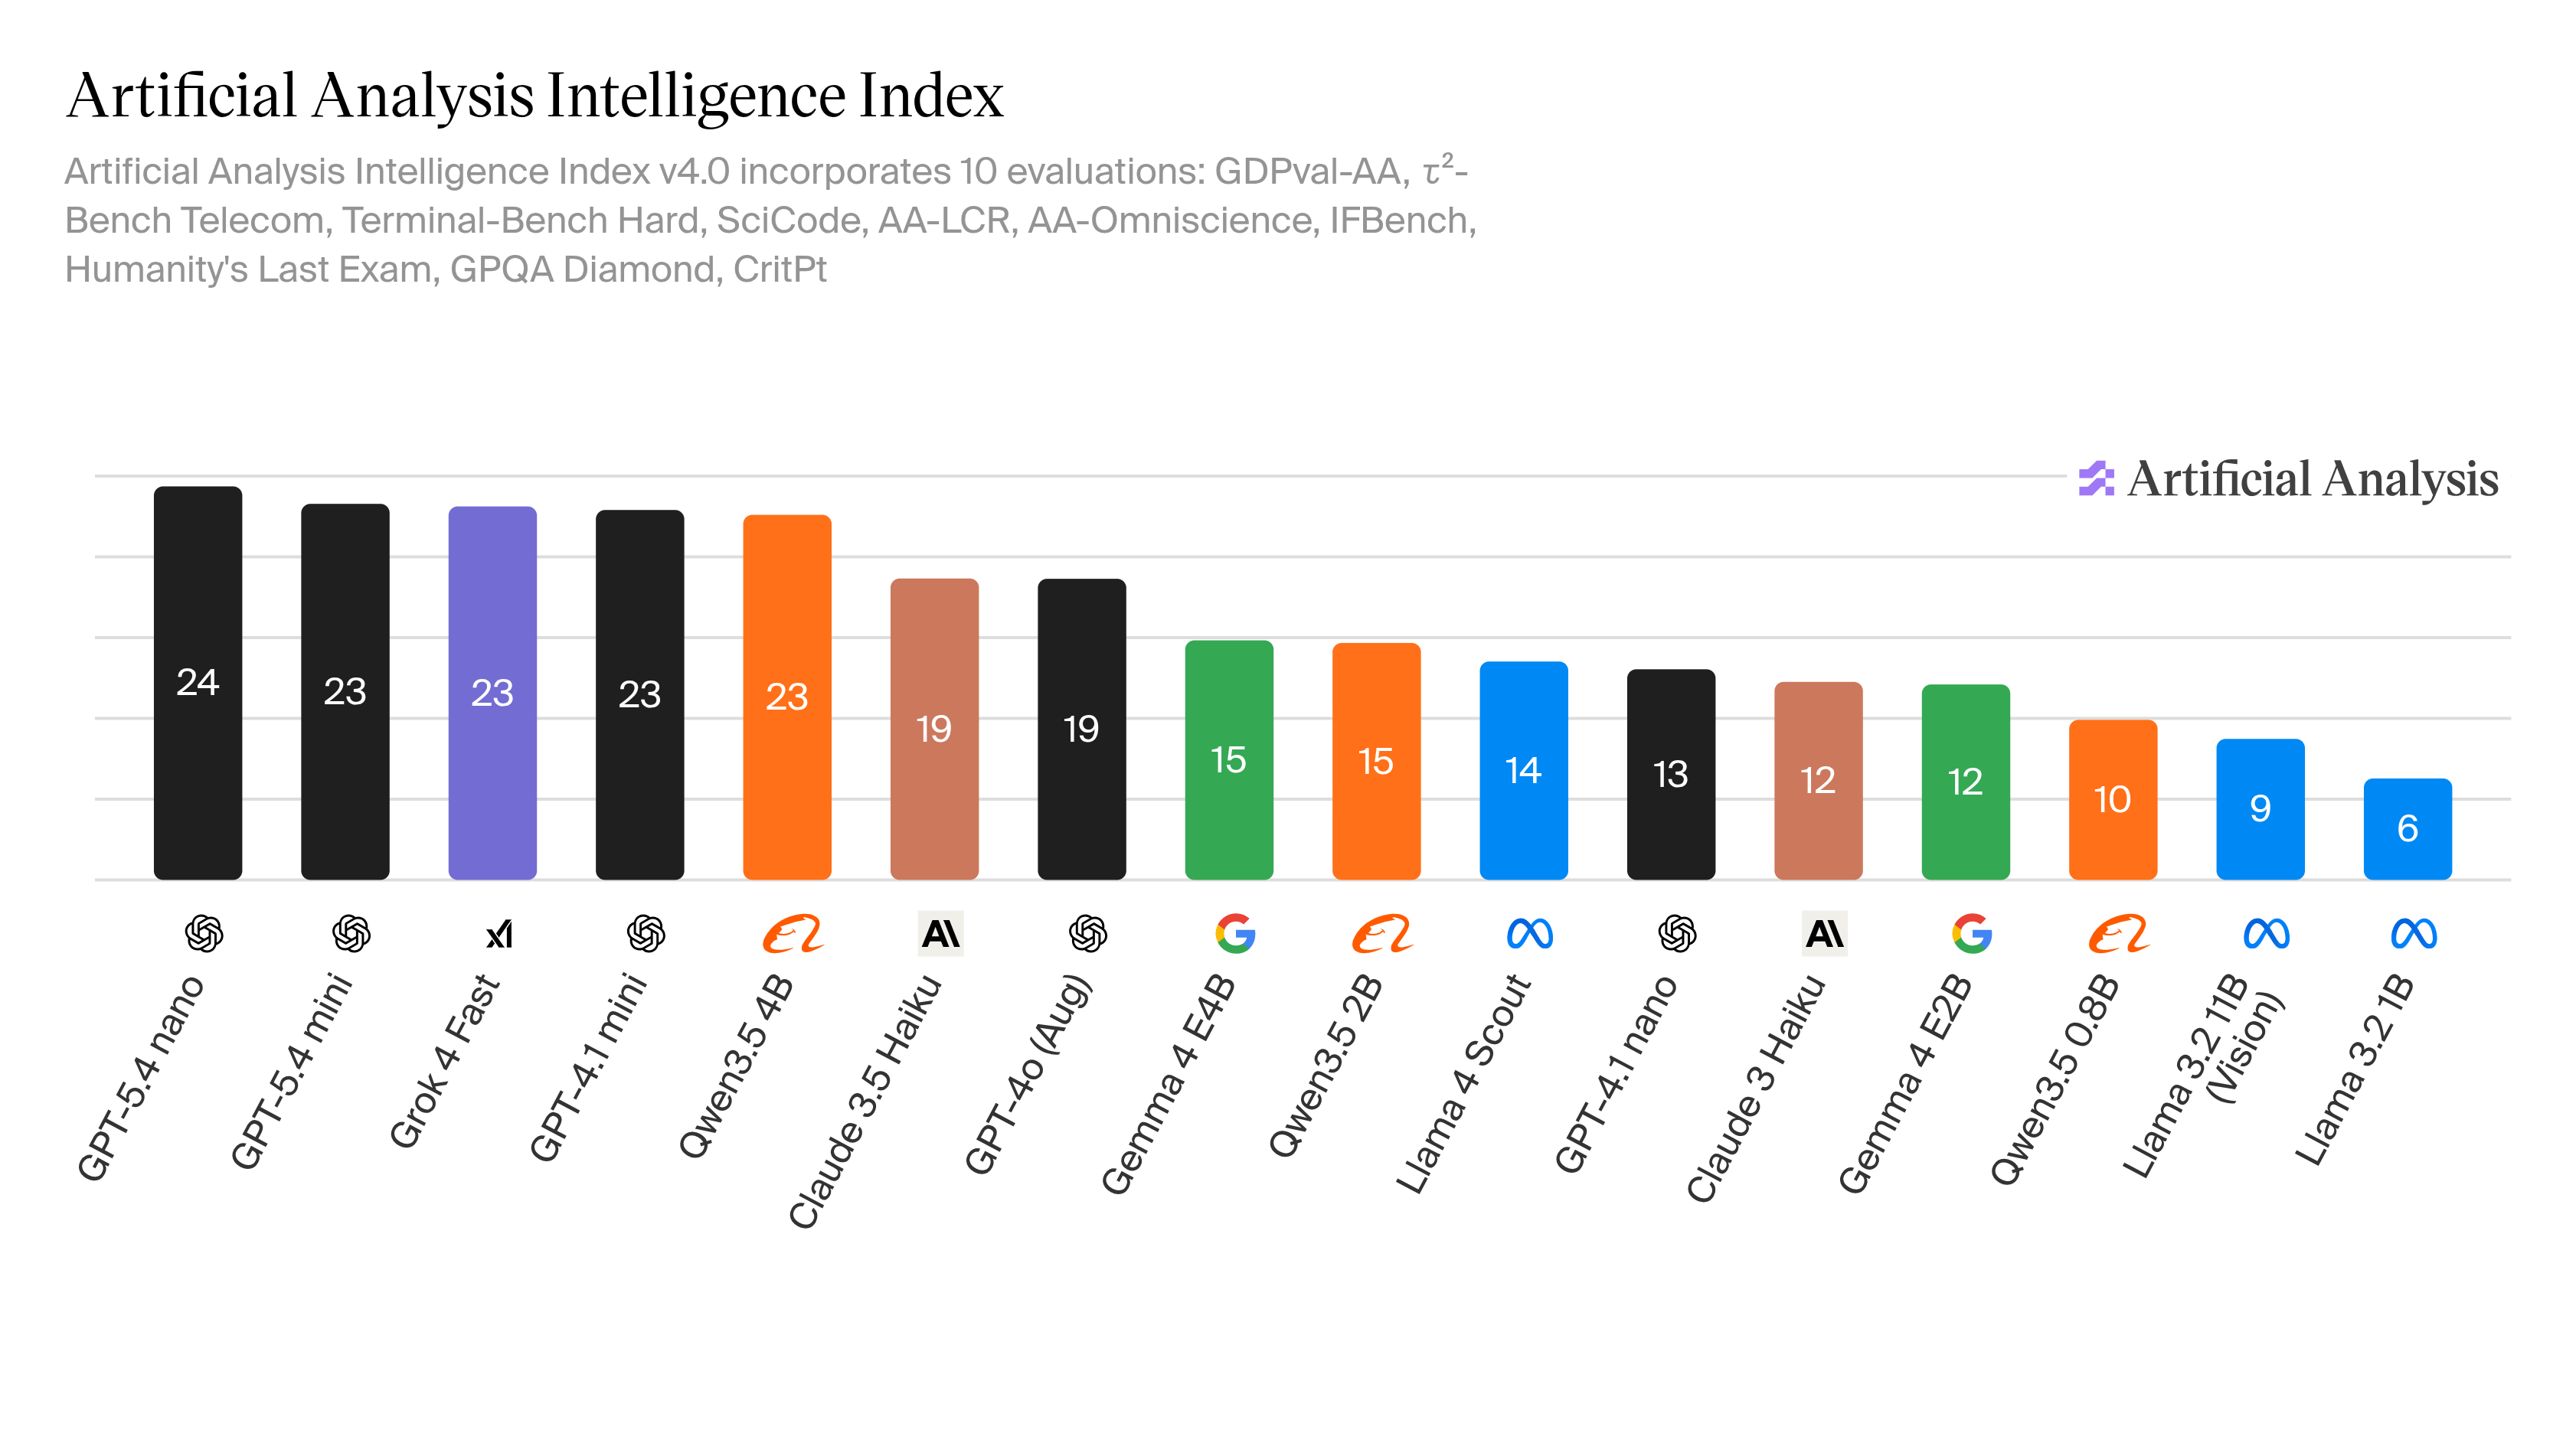
\includegraphics[width=1\linewidth]{leaderboard.png}
\caption{Gemma 4 and Qwen 3.5 at very small parameter sizes consistently beat prior Llama models of the same weight classes and approach performance of proprietary small model variants from last year \cite{artificialanalysis2026}}
\label{fig:artificial-analysis-leaderboard}
\end{figure}

\begin{figure}[H]
\centering
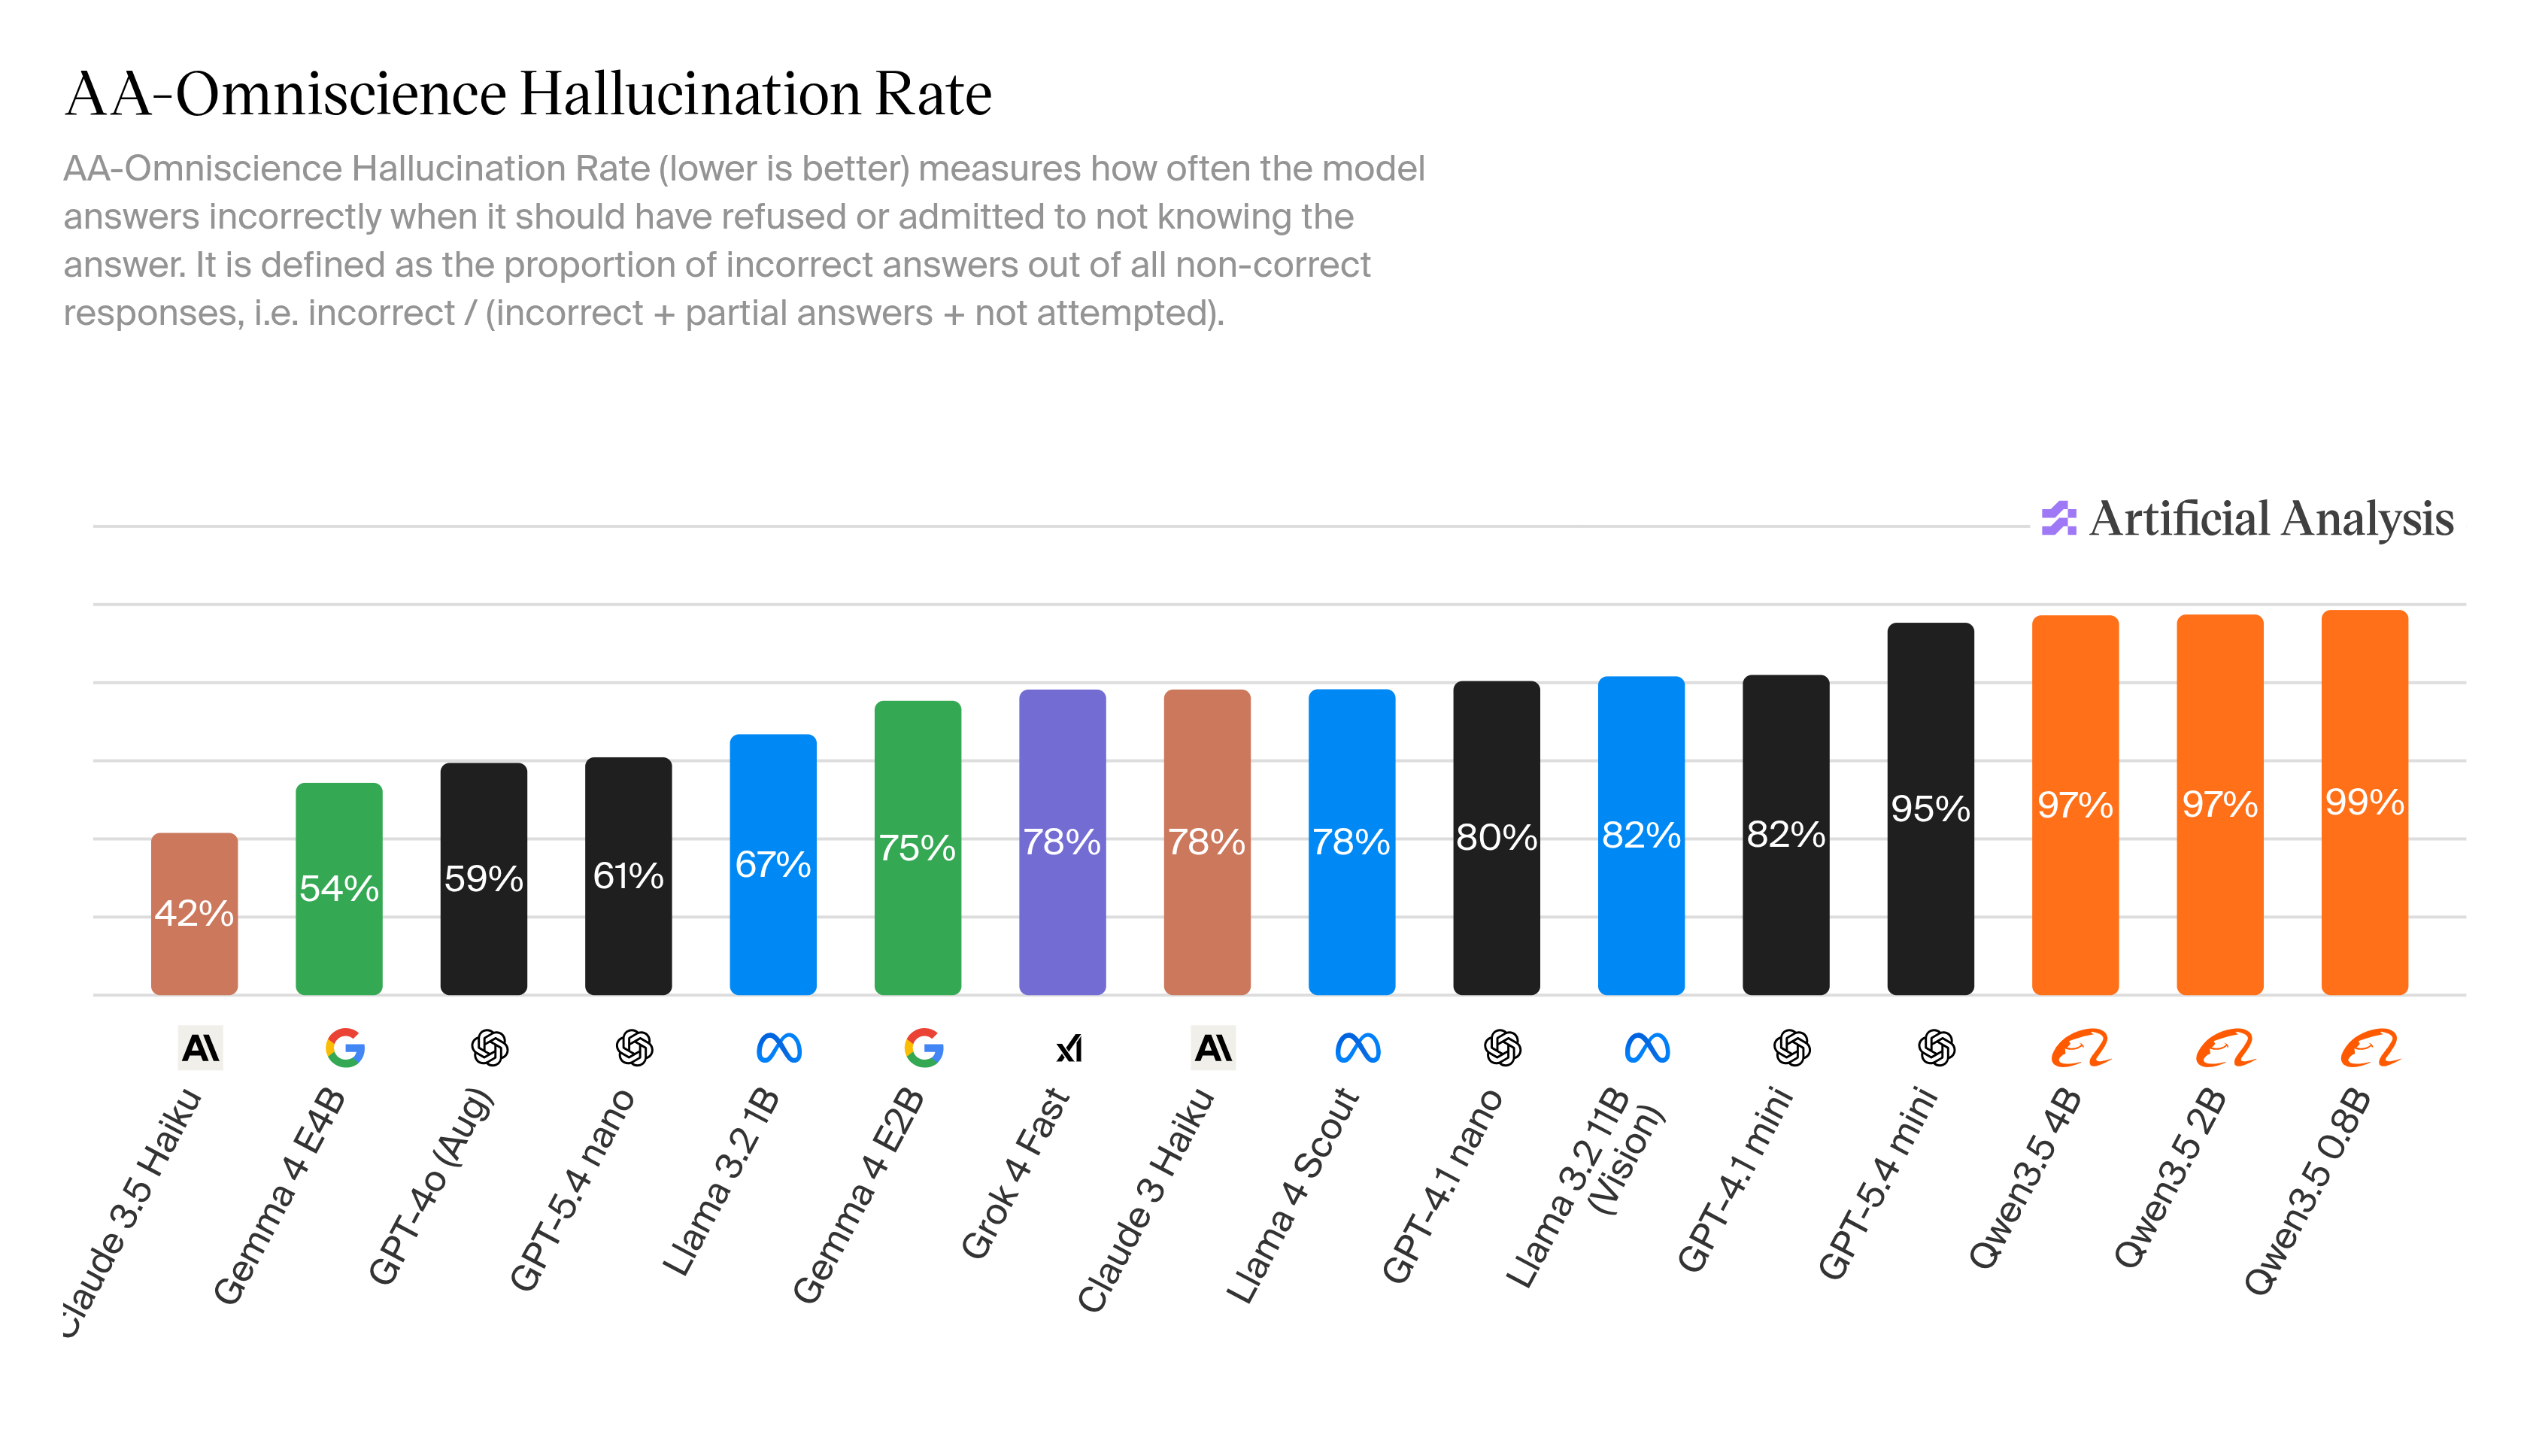
\includegraphics[width=1\linewidth]{hallucinations.png}
\caption{Gemma 4 has a competitive edge in hallucination reduction \cite{artificialanalysis2026}.}
\label{fig:artificial-analysis-hallucinations}
\end{figure}

\begin{figure}[H]
\centering
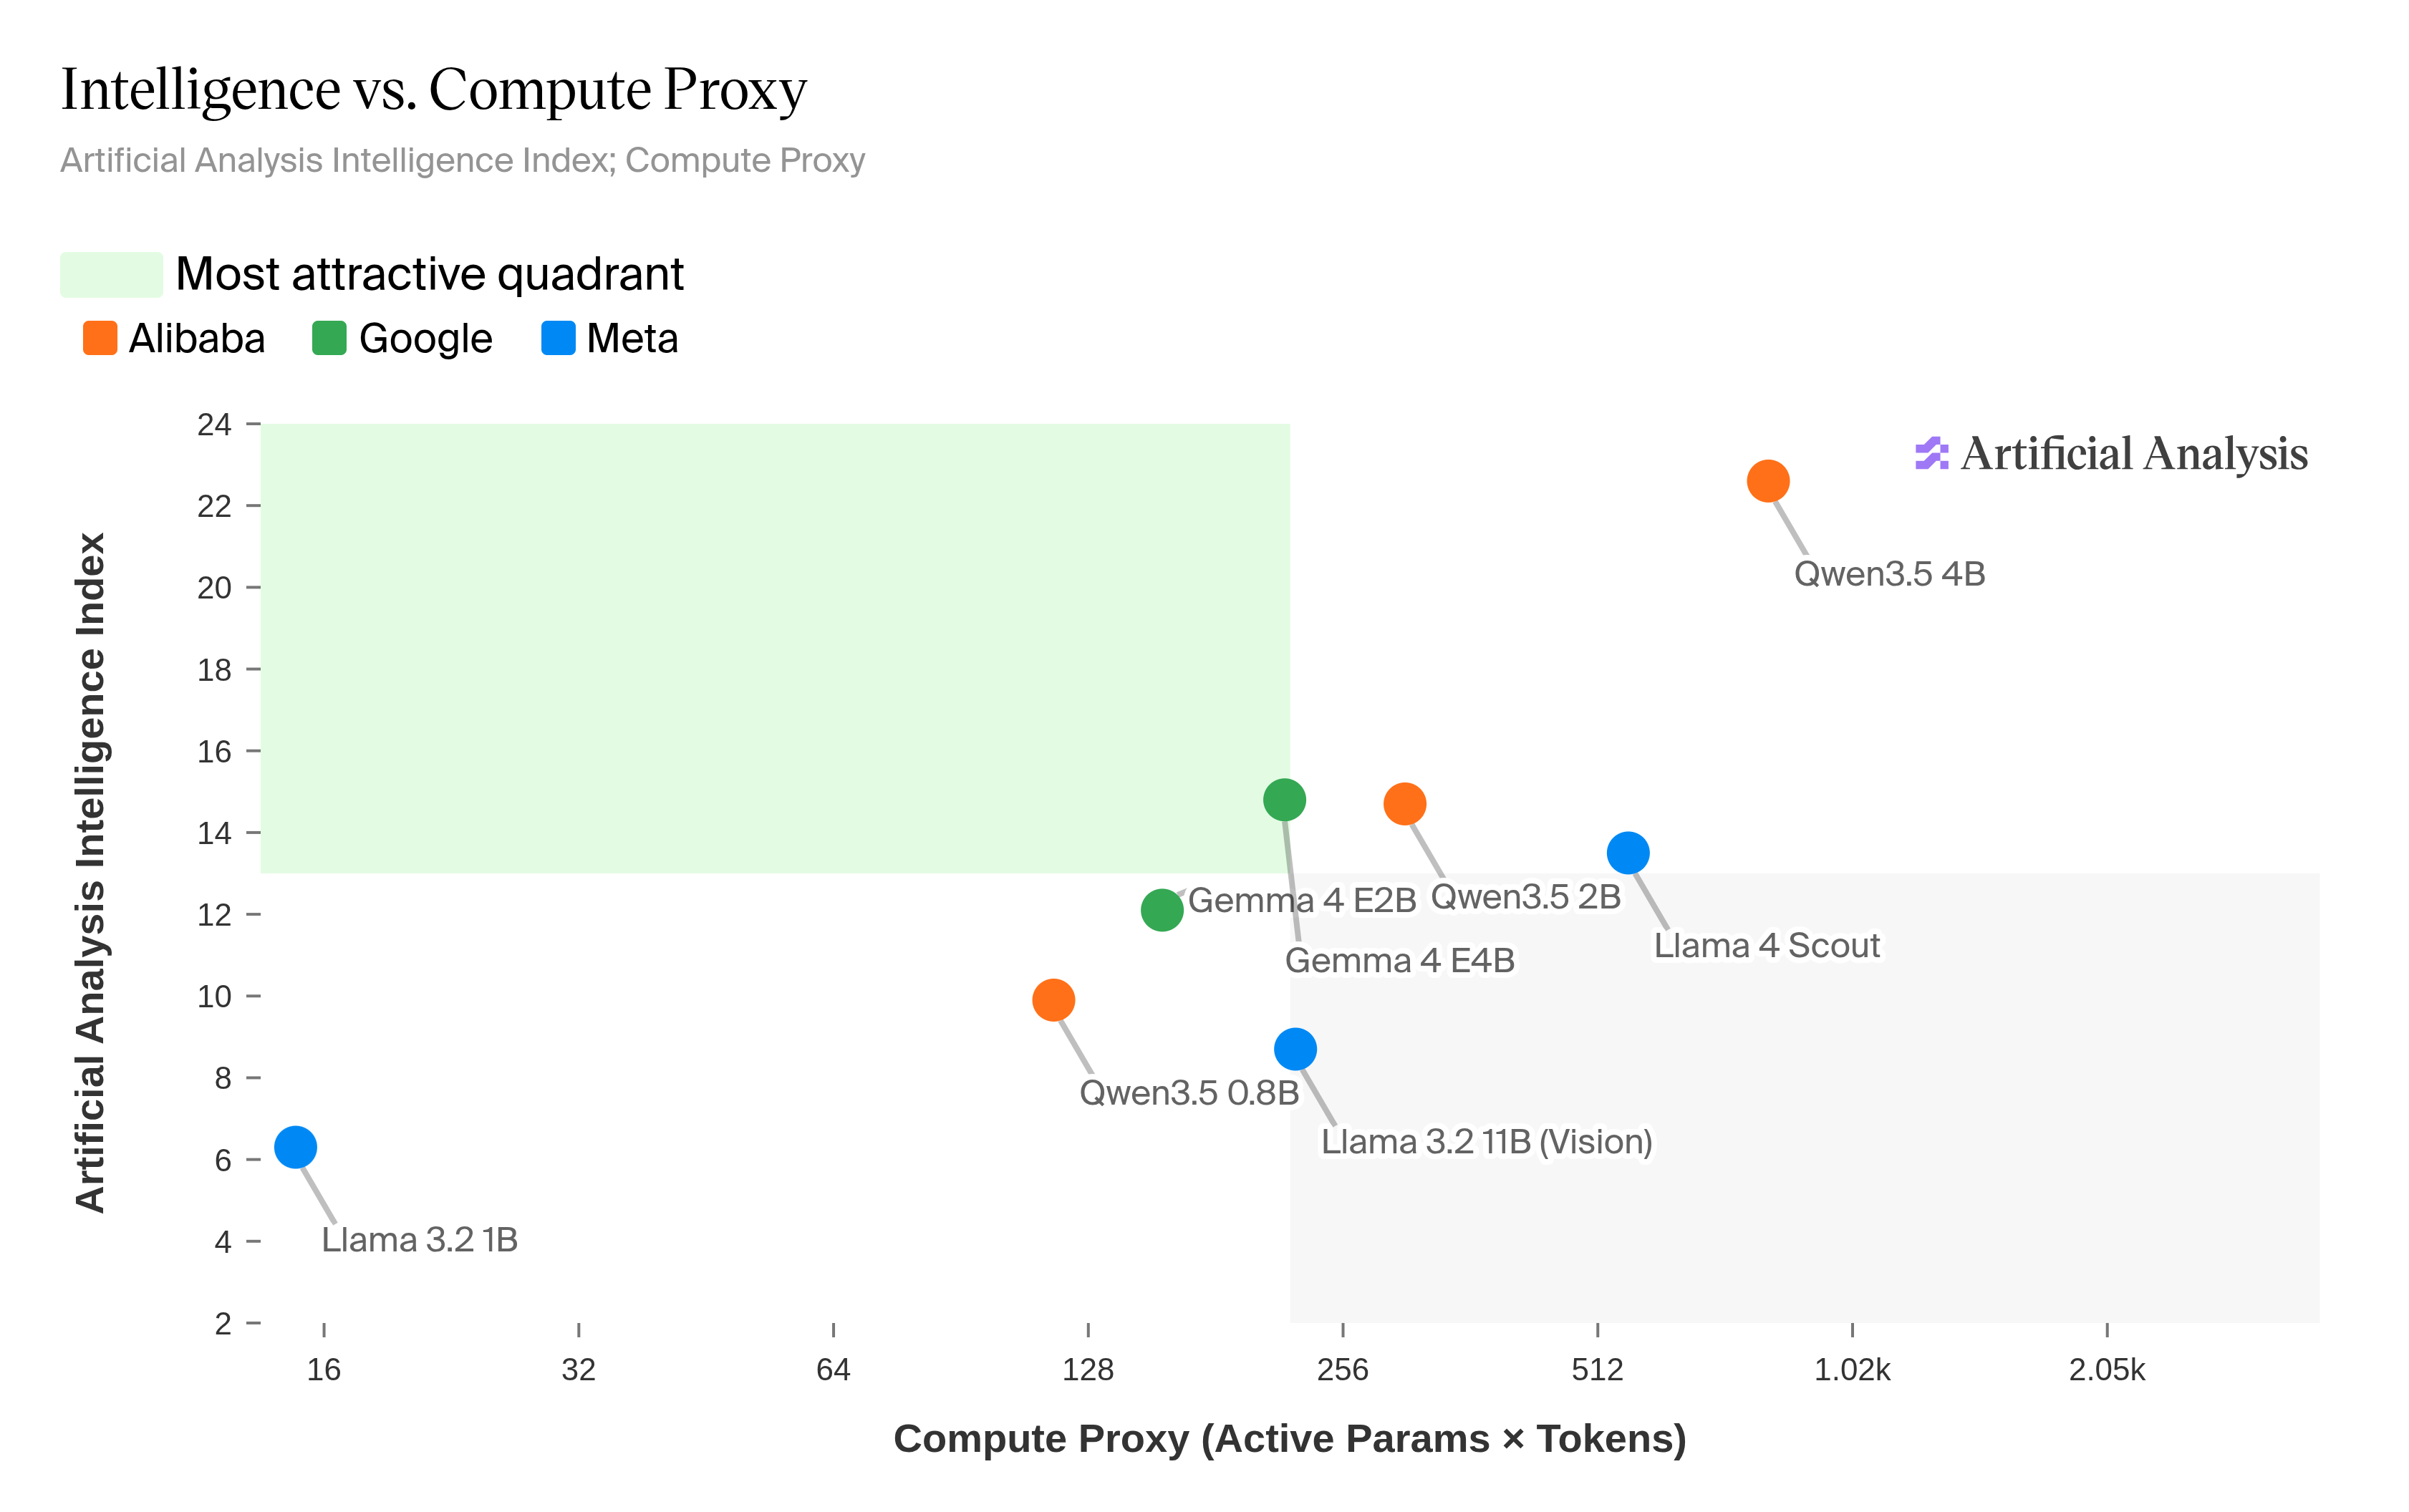
\includegraphics[width=1\linewidth]{compute.png}
\caption{Gemma 4 especially has an advantage in terms of compute usage. \cite{artificialanalysis2026}. The author of this paper was able to run it on a 2024 Intel Core 7 Laptop with 32 GB RAM and no graphics card with minimal latency at both E4B and E2B sizes}
\label{fig:artificial-analysis-compute}
\end{figure}

This project focuses specifically on simple sentiment classification (POSITIVE, NEGATIVE, NEUTRAL).

\section{Literature Review}
Gupta's Comprehensive Study on Sentiment Analysis gives a good explanation of the state of affairs as of a few years ago during the emergence of GPT and BERT models for sentiment analysis as compared to CNNs and RNNs. The affects of sarcasm and irony are noted as unique challenges that maybe LLMs and others could help with. \cite{gupta2024comprehensive}

\subsection{Sentiment Analysis in the Era of LLMs: A Reality Check}\cite{zhang2024realitycheck}

\subsection{Fine-tuned LLMs for Sentiment Prediction}\cite{dave2023finetunedllms}

\subsection{How to Do Sentiment Analysis With LLMs}\cite{burchell2024llmssentiment}

\subsection{Public Health Discussions on Social Media}\cite{gandy2025publichealth}

\subsection{LLMs for Vaccine Sentiment and Hesitancy}\cite{annan2025vaccine}

\subsection{COP9 Tweet Sentiment Analysis}\cite{elmitwalli2024cop9}

\subsection{LLMs vs. Traditional Sentiment Tools in Psychology}\cite{kandala2025llmsvstraditional}

\subsection{medRxiv Source}\cite{medrxiv2024preprint}

\subsection{MDPI Source}\cite{mdpi2024article}

\section{Methodology}
We benchmarked six sentiment models: Gemma 4 E2B \cite{gemma4}, Qwen3.5 0.8B Q4 and Qwen3.5 2B Q4 \cite{qwen35}, BERTweet Sentiment \cite{bertweet}, Reviews-SST2 \cite{socher2013recursive}, and Twitter-RoBERTa \cite{barbieri2020tweeteval}. Evaluation used three datasets: Instagram comments (56 samples), Kaggle Reviews (2000 samples), and a mixed-domain Kaggle Sentiment set (499 samples). The Kaggle movie-review data is based on the Large Movie Review Dataset (IMDb) \cite{maas2011learning}.

\section{Results}
Presentation of the findings, including tables, figures, and statistical analyses.

\subsection{Instagram - 56 samples}

\begin{table}[H]
\centering
\begin{tabular}{@{}lcc@{}}
\toprule
\textbf{Model} & \textbf{Accuracy} & \textbf{Latency (s)} \\
\midrule
Gemma 4 E2B & 60.71\% & 0.0930 \\
Qwen3.5 0.8B Q4 & 28.57\% & 0.2128 \\
Qwen3.5 2B Q4 & 28.57\% & 0.5344 \\
BERTweet Sentiment & 60.71\% & 0.0081 \\
Reviews-SST2 & 46.43\% & 0.0035 \\
Twitter-RoBERTa & 60.71\% & 0.0062 \\
\bottomrule
\end{tabular}
\caption{Benchmark results for Instagram dataset (56 samples).}
\label{tab:benchmark-results-instagram}
\end{table}

\begin{figure}[H]
\centering

\includegraphics[width=0.85\linewidth]{report_charts/report_accuracy_instagram_comments_test.png}
\caption{Accuracy by model for Instagram.}
\label{fig:accuracy-instagram}
\end{figure}

\begin{figure}[H]
\centering

\includegraphics[width=0.85\linewidth]{report_charts/report_compute_cost_instagram_comments_test.png}
\caption{Latency by model for Instagram.}
\label{fig:latency-instagram}
\end{figure}

\subsection{Kaggle Reviews - 2000 samples}

\begin{table}[H]
\centering
\begin{tabular}{@{}lcc@{}}
\toprule
\textbf{Model} & \textbf{Accuracy} & \textbf{Latency (s)} \\
\midrule
Gemma 4 E2B & 63.00\% & 0.0851 \\
Qwen3.5 0.8B Q4 & 65.00\% & 0.1559 \\
Qwen3.5 2B Q4 & 65.00\% & 0.3159 \\
BERTweet Sentiment & 63.00\% & 0.0060 \\
Reviews-SST2 & 68.00\% & 0.0031 \\
Twitter-RoBERTa & 65.00\% & 0.0060 \\
\bottomrule
\end{tabular}
\caption{Benchmark results for Kaggle Reviews dataset (2000 samples).}
\label{tab:benchmark-results-kaggle-reviews}
\end{table}

\begin{figure}[H]
\centering

\includegraphics[width=0.85\linewidth]{report_charts/report_accuracy_kaggle_reviews_dolbokostya_subset.png}
\caption{Accuracy by model for Kaggle Reviews.}
\label{fig:accuracy-kaggle-reviews}
\end{figure}

\begin{figure}[H]
\centering
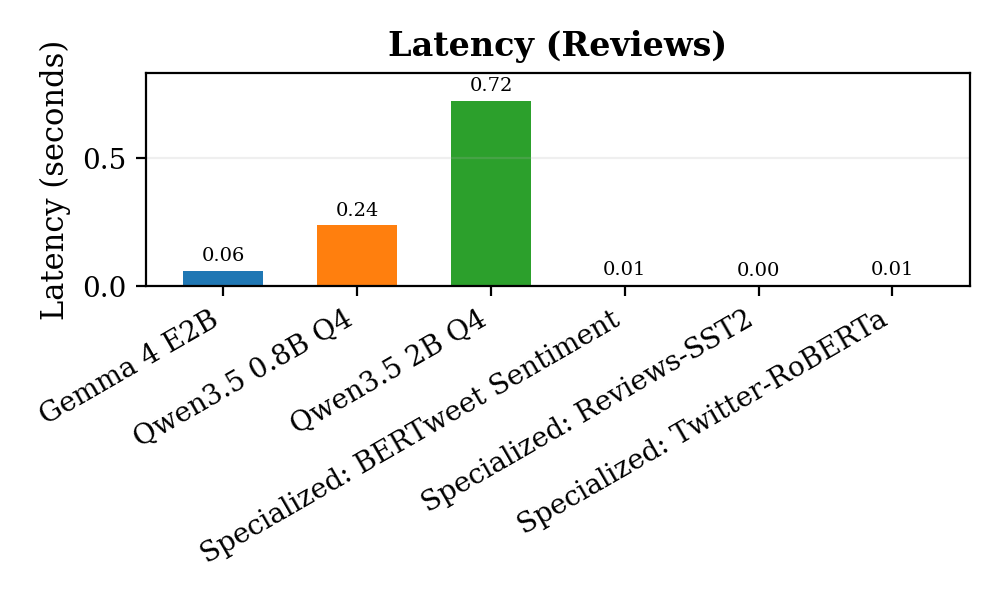
\includegraphics[width=0.85\linewidth]{report_charts/report_compute_cost_kaggle_reviews_dolbokostya_subset.png}
\caption{Latency by model for Kaggle Reviews.}
\label{fig:latency-kaggle-reviews}
\end{figure}

\subsection{Mixed Domain - 499 samples}

\begin{table}[H]
\centering
\begin{tabular}{@{}lcc@{}}
\toprule
\textbf{Model} & \textbf{Accuracy} & \textbf{Latency (s)} \\
\midrule
Gemma 4 E2B & 73.21\% & 0.0976 \\
Qwen3.5 0.8B Q4 & 33.87\% & 0.2421 \\
Qwen3.5 2B Q4 & 32.26\% & 0.4828 \\
BERTweet Sentiment & 71.94\% & 0.0059 \\
Reviews-SST2 & 50.70\% & 0.0033 \\
Twitter-RoBERTa & 71.94\% & 0.0061 \\
\bottomrule
\end{tabular}
\caption{Benchmark results for Kaggle Sentiment dataset (499 samples).}
\label{tab:benchmark-results-kaggle-sentiment}
\end{table}

\begin{figure}[H]
\centering

\includegraphics[width=0.85\linewidth]{report_charts/report_accuracy_kaggle_sentiment_analysis_mdismielhossenabir.png}
\caption{Accuracy by model for Kaggle Sentiment.}
\label{fig:accuracy-kaggle-sentiment}
\end{figure}

\begin{figure}[H]
\centering

\includegraphics[width=0.85\linewidth]{report_charts/report_compute_cost_kaggle_sentiment_analysis_mdismielhossenabir.png}
\caption{Latency by model for Kaggle Sentiment.}
\label{fig:latency-kaggle-sentiment}
\end{figure}

\section{Discussion}
Interpretation of the results, implications, and relation to previous research.

\section{Conclusion}
Summary of the main findings, limitations of the study, and suggestions for future research.

% This will automatically generate the References section. You do not need to add a References section manually.
%\nocite{*}
\bibliographystyle{bib_styles/acl_natbib_no_note}
\bibliography{biblio}

\end{document}
